\section{Proposed Method: CUE}
\label{sec:method}
\begin{figure*}[t]
  \centering
  % \vspace{-1em}
  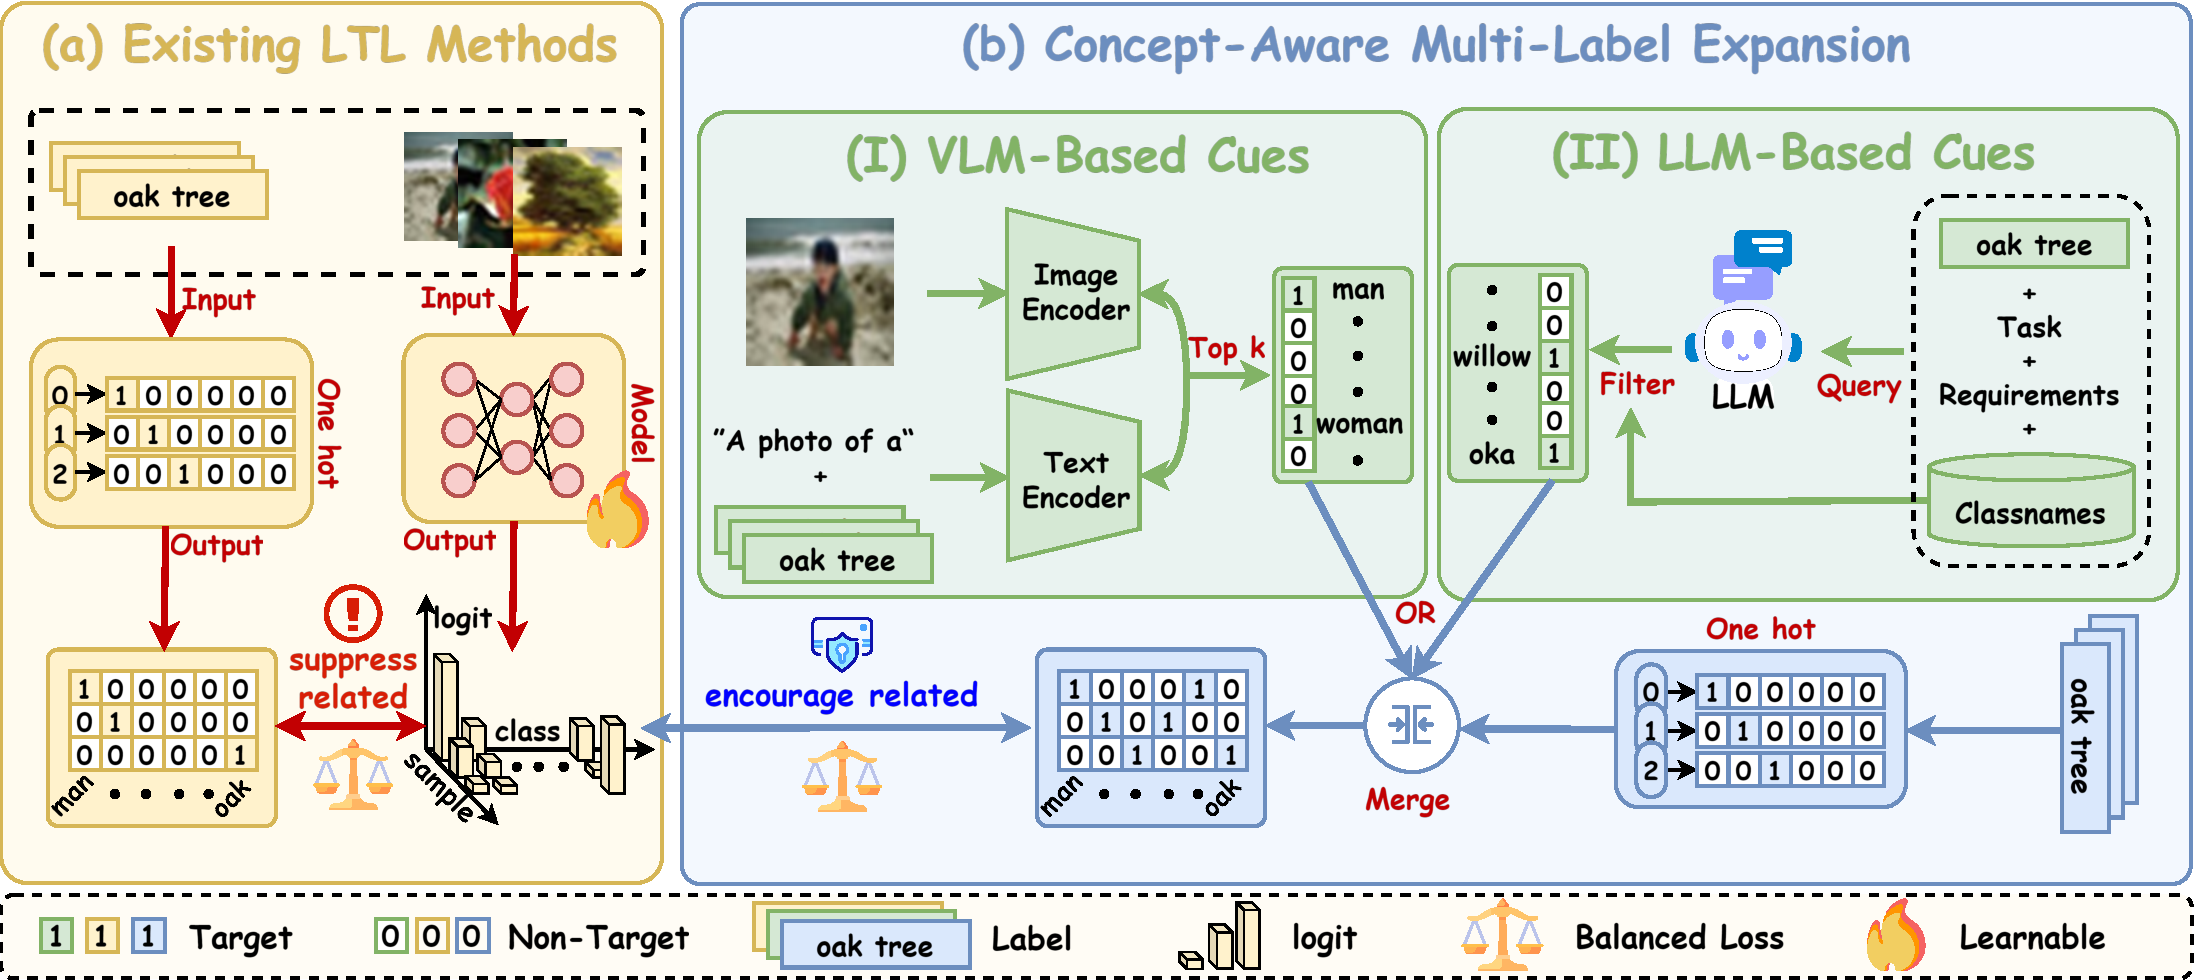
\includegraphics[width=\textwidth]{img/method_v4.pdf}
  \vspace{-1.6em}
    \caption{\textbf{Overall framework.}
    This figure illustrates the overall structure of our approach compared with the existing long-tailed learning methods.
    (a) \textit{Existing LTL methods} rely on a single-label balanced loss, which tends to suppress semantically related categories and bias learning toward head classes, often leading to concept confusion.
    (b) \textit{CUE} augments the main balanced loss with two concept-aware cues: (I) VLM-based instance-level cues and (II) LLM-based class-level cues. By jointly optimizing these cues with the BLA objective, CUE encourages learning from semantically related categories rather than suppressing them, effectively alleviating concept confusion.}
    \label{fig:overview}
    \vspace{-1.3em}
\end{figure*}

As discussed in Sec.~\ref{sec:intro}, fine-tuning foundation models on long-tailed data often amplifies concept confusion. We attribute this phenomenon to the exclusivity of single-label supervision, which suppresses the shared representations among semantically related categories and distorts the inter-class relationships established during pre-training. To address this issue, our framework, shown as Fig.~\ref{fig:overview}, extends the typical long-tailed learning paradigm by adding a plug-and-play module, CUE, which explicitly mitigates such confusion through joint supervision from VLM-based and LLM-based cues. These cues provide complementary visual and semantic guidance, enabling the model to preserve the pre-trained knowledge while adapting to the new  domain during fine-tuning. 
% The detailed method process is summarized in Algorithm~\textcolor[HTML]{367DBD}{1} in the Appendix~\textcolor[HTML]{367DBD}{A}.

\subsection{Preliminaries}
\label{sec:prelim}
\noindent \textbf{Notation.} We denote the training set with $N$ samples as $\mathcal{D}=\{(\mathbf{x}_i, y_i)\}_{i=1}^N$, where $\mathbf{x}_i$ indicates the $i$-th image sample and $y_i$ denotes its corresponding label. 
Let $n_c$ represent the number of samples in class $c$, and $C$ be the total number of classes. Given an input image $\mathbf{x}$, the model outputs a logit vector $\boldsymbol{\theta}(\mathbf{x}) \in \mathbb{R}^C$ corresponding to $C$ categories, where $\theta_y(\mathbf{x})$ denotes the logit corresponding to the label $y$.
The empirical class prior is given by $\pi_c = n_c / \sum_j n_j$.  
% \vspace{0.5em}

\noindent \textbf{Logit Adjustment.}
Logit Adjustment~\cite{menon2021longtail} rebalances long-tailed data by correcting the class posterior through Bayes’ rule. 
Since $\mathbb{P}(y|\mathbf{x})\!\propto\!\mathbb{P}(\mathbf{x}|y)\mathbb{P}(y)$, standard training on imbalanced data implicitly optimizes $\mathbb{P}_{\text{train}}(y|\mathbf{x})\!\propto\!\mathbb{P}(\mathbf{x}|y)\mathbb{P}_{\text{train}}(y)$, 
which biases predictions toward frequent classes. 
Assuming $\mathbb{P}(\mathbf{x}|y)$ remains unchanged between training and test distributions, 
a balanced posterior can be approximated as 
$\mathbb{P}_{\text{bal}}(y|\mathbf{x})\!\propto\!\mathbb{P}_{\text{train}}(y|\mathbf{x})/\mathbb{P}_{\text{train}}(y)
\!\propto\!\mathrm{softmax}(\theta_y(\mathbf{x})-\log\mathbb{P}_{\text{train}}(y))$.
Introducing a temperature $\tau$ yields the general form 
$\theta'_y(\mathbf{x})=\theta_y(\mathbf{x})-\tau\log\mathbb{P}_{\text{train}}(y)$, 
which can be applied during training to mitigate class imbalance. 
Since our framework adopts multi-label expansion, fair calibration between positive and negative samples is essential. 
To address this, we further extend the standard binary cross-entropy loss with same prior logit shift, 
resulting in a \emph{Binary Logit Adjustment (BLA)} formulation that aligns with our VLM- and LLM-based supervision. 
% A detailed derivation is provided in Appendix~\textcolor[HTML]{367DBD}{B}.










% In our framework, we start from a balanced single-label baseline (e.g., LA~\cite{menon2021longtail}) and extend it with \textbf{CUE}, which introduces multi-label supervision to capture visually and semantically confusable classes around the ground truth. 
% For fine-tuning scenarios, we employ a pre-trained CLIP backbone and freeze its parameters during training.
% ToDo: 这里根据情况 添加from scretch的内容
% ToDo: 是不是要加微调 以及 Logit adjustment 的相关Preliminaries

\subsection{VLM-Based Instance-Level Cues}
\label{sec:vlm_prior}
Considering that visual language model (VLM) naturally provides instance-level cues, we use their zero-shot predictions to capture potential cross-class confusion, thereby mitigating instance-level concept confusion. Specifically, for each training image $\mathbf{x}_i$, we compute its zero-shot prediction scores ${\theta}^{\text{zs}}(\mathbf{x}_i)$ by measuring the cosine similarities between the CLIP image embedding of $\mathbf{x}_i$ and the text prototypes generated from the pre-trained CLIP model using the standard prompt ``a photo of a [CLASS].'', and identify the Top-$k$ non-ground-truth categories that the model considers most similar:
\begin{equation}
\mathcal{T}^{\text{zs}}(x_i) = \text{Top-}k\Big(\operatorname*{argsort}_{y \neq y_i}\, {\theta}^{\text{zs}}_y(\mathbf{x}_i)\Big),
\end{equation}
where ${\theta}^{\text{zs}}_y(\mathbf{x}_i)$ denotes the zero-shot prediction logit of label $y$ obtained from the frozen CLIP model, and $\mathcal{T}^{\text{zs}}(\mathbf{x}_i)$ represents the Top-$k$ semantically similar non-ground-truth classes according to pre-trained embedding space of CLIP, which serve as additional visual and conceptual cues of $y_i$. 
To incorporate this relational cue into training, we augment the supervision signal by converting them into a binary multi-label target:
\begin{equation}
\tilde{t}^{\text{zs}}_{i} =
\begin{cases}
1, & c \in \{y_i\} \cup \mathcal{T}^{\text{zs}}(\mathbf{x}_i), \\
0, & \text{otherwise,}
\end{cases}
\end{equation}
where $\tilde{t}^{\text{zs}}_{i}$ denotes the enhanced multi-label supervision for sample $\mathbf{x}_i$.
These instance-level cues effectively preserve the local class neighborhood discovered during pre-training, maintaining the intrinsic visual structure learned by CLIP. It encourages the model to recognize visually correlated categories and maintain coherent representations across related classes, thereby mitigating concept confusion.

\subsection{LLM-Based Class-Level Cues}
\label{sec:llm_prior}

Similar to the instance-level cues derived from VLM, we further incorporate class-level semantic cues by leveraging large language model (LLM) to uncover relationships among original categories.
To mitigate concept confusion at the class level, we build for each class $c$ an offline neighbor set $\mathcal{N}^{\text{llm}}(c)$ using LLM. The LLM is prompted with the complete label vocabulary as the only candidate set and instructed to select semantic neighbors strictly from it. In practice, the LLM may still produce occasional out-of-vocabulary names, so we simply filter these out during post-processing to ensure all neighbors remain within the original label space.

\begin{figure}[h]
\centering
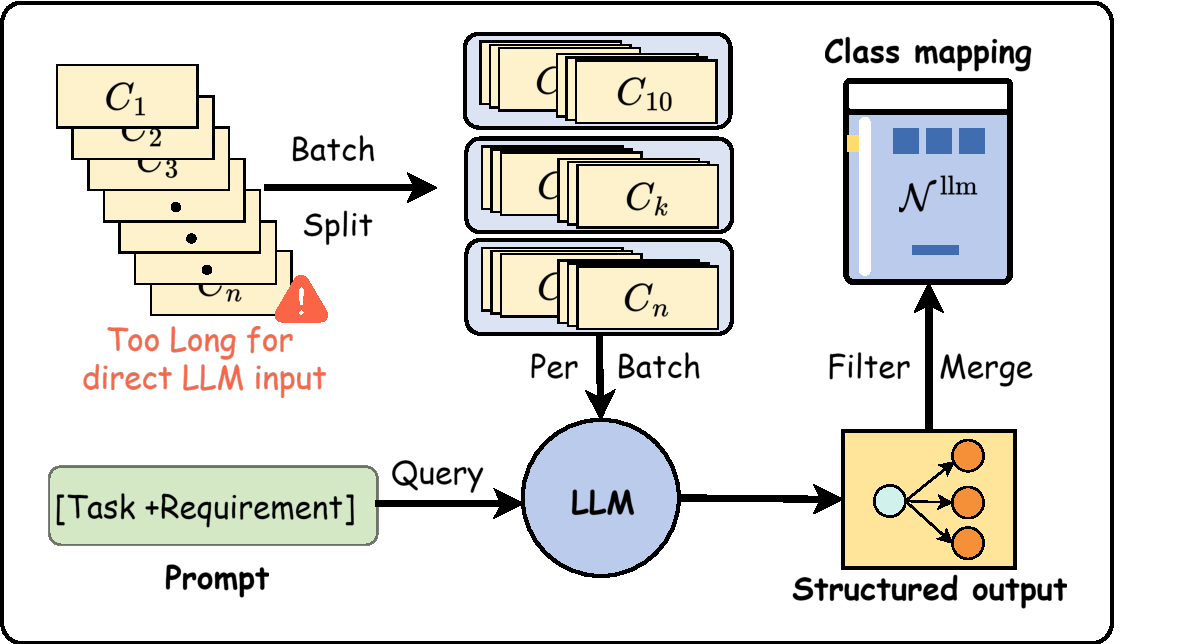
\includegraphics[width=\linewidth]{img/llm_pipline_v4.pdf}
\vspace{-1.0em}
\caption{\textbf{Construction pipeline of the LLM-based class-level cues}. This figure shows the process used to obtain the LLM-based semantic neighbor graph $\mathcal{N}^{\text{llm}}$.
}
\label{fig:llm_pipeline}
\vspace{-1.5em}
\end{figure}

However, directly prompting the entire label list tends to exceed the effective working range of the LLM, causing it to skip or collapse intermediate classes. As a result, the model exhibits degraded semantic quality, producing coarse or noisy relations instead of fine-grained confusion patterns. To ensure stable and comprehensive neighbor discovery across the full vocabulary, we design a \emph{batched prompting and filtering pipeline}: (i) the full label list is divided into batches, and each query is \emph{constrained} to return JSON mappings from class names to their nearest semantic neighbors strictly within the given subset; (ii) the batched outputs are merged and post-filtered to remove out-of-list, ambiguous, and duplicate entries, before aligning the class names to label indices (as shown in Fig.~\ref{fig:llm_pipeline}). Each batch follows a standardized instruction template to ensure consistent and structured LLM responses.



During training, each sample $(\mathbf{x}_i, y_i)$ receives additional class-level supervision constructed from its semantic neighbors:
\begin{equation}
\tilde{t}^{\text{llm}}_{i} =
\begin{cases}
1, & c \in \{y_i\} \cup \mathcal{N}^{\text{llm}}(y_i), \\
0, & \text{otherwise.}
\end{cases}
\end{equation}
where $\tilde{t}^{\text{llm}}_{i}$ denotes the augmented class-level multi-label target for sample $\mathbf{x}_i$, 
and $\mathcal{N}^{\text{llm}}(y_i)$ represents the set of neighbor classes of $y_i$ 
obtained from the LLM-generated class-level cues. These class-level cues capture broader semantic associations and complement the instance-level visual cues by introducing higher-level contextual structure.
They encourage the model to learn coherent representations across semantically related categories, thereby reducing concept confusion under long-tailed distributions.


% \begin{equation}
% \begin{split}
% \mathcal{L}
% = &~ \underbrace{\mathcal{L}^{\text{LA}}(x_i, y_i)}_{\text{baseline}} \\
% & + \lambda_{\text{zs}} 
%   \underbrace{\mathcal{L}^{\text{BLA}}(x_i, \tilde{\mathbf{t}}^{\text{zs}}_i)}_{\text{VLM prior}}
%   + \lambda_{\text{llm}} 
%   \underbrace{\mathcal{L}^{\text{BLA}}(x_i, \tilde{\mathbf{t}}^{\text{llm}}_i)}_{\text{LLM prior}},
% \end{split}
% \label{eq:overall_loss}
% \end{equation}

\subsection{Training Objectives}
\label{sec:objective}
Our training objective integrates the instance-level and class-level cues into a unified optimization framework that balances data-driven and cue-guided supervision. 
Specifically, we employ a single-label logit-adjusted (LA) loss and two multi-label binary logit-adjusted (BLA) terms corresponding to the VLM-based and LLM-based cues:
\begin{equation}
\begin{aligned}
\mathcal{L}
= &
~\underbrace{
  \colorbox{gray!15}{$\mathcal{L}^{\text{LA}}(\mathbf{x}_i, y_i)$}
}_{\text{baseline}}
+ \lambda_{\text{zs}}
  \underbrace{
  \colorbox{blue!10}{$\mathcal{L}^{\text{BLA}}(\mathbf{x}_i, \tilde{\mathbf{t}}^{\text{zs}}_i)$}
}_{\text{VLM cue}}
\\[2pt]
&+ \lambda_{\text{llm}}
  \underbrace{
  \colorbox{green!10}{$\mathcal{L}^{\text{BLA}}(\mathbf{x}_i, \tilde{\mathbf{t}}^{\text{llm}}_i)$}
}_{\text{LLM cue}},
\end{aligned}
\label{eq:overall_loss}
\end{equation}
where $\lambda_{\text{zs}}$ and $\lambda_{\text{llm}}$ are weighting coefficients for the two prior-guided terms, and 
$\tilde{\mathbf{t}}^{\text{zs}}_i$ and $\tilde{\mathbf{t}}^{\text{llm}}_i$ denote the multi-label supervision targets derived from the VLM-based instance-level and LLM-based class-level cues.

% \vspace{0.5em}

\noindent \textbf{Logit-Adjustment (LA).} The baseline loss adopts class-balanced logit adjustment, which introduces a log-prior shift with temperature~$\tau$:
\begin{equation}
\begin{split}
\theta'_c(\mathbf{x}) &= \theta_c(\mathbf{x}) + \tau \log \pi_c, \\
\mathcal{L}^{\text{LA}} 
&= -\log
\frac{\exp\!\big(\theta'_{y_i}(\mathbf{x}_i)\big)}
{\sum_{c}\exp\!\big(\theta'_{c}(\mathbf{x}_i)\big)},
\end{split}
\end{equation}
where $\pi_c$ denotes the empirical class prior defined in Sec.~\ref{sec:prelim}.
This formulation mitigates class imbalance by reducing the dominance of frequent classes through prior-dependent re-weighting.


% \vspace{0.5em}

\noindent \textbf{Binary Logit-Adjustment (BLA).}
For multi-label supervision, we apply a similar prior logit adjustment before the sigmoid activation:
\begin{equation}
\begin{split}
\tilde\theta_c(\mathbf{x}) &= \theta_c(\mathbf{x}) + \tau_{\text{b}}\log \pi_c, \\
\mathcal{L}^{\text{BLA}}
&= -\frac{1}{C}\sum_{c=1}^{C}\Big[
\tilde{t}_{i,c}\log\sigma\!\big(\tilde\theta_c(\mathbf{x}_i)\big) \\
&\qquad
+~(1-\tilde{t}_{i,c})\log\!\big(1-\sigma\!\big(\tilde\theta_c(\mathbf{x}_i)\big)\big)
\Big],
\end{split}
\end{equation}
where $\sigma(\cdot)$ denotes the sigmoid function and $\tilde{t}_{i,c}\!\in\!\{0,1\}$ is the augmented supervision target for class $c$.

By jointly optimizing these objectives, the model mitigates the effect of single-label exclusivity by encouraging semantically related categories to share representations, leading to more balanced and coherent learning under long-tailed distributions.


% ToDO： \paragraph{Complexity and Inference.}
% The VLM prior adds a single frozen forward pass; the LLM prior is precomputed offline and adds no runtime cost. Inference remains standard $\arg\max_c {\theta}_c(x)$ without extra heads.




% ToDo: \subsection{addtion analize}
% \label{sec:anali}
% \subsection{Data-Specific Transformation Strategy}
% Beyond the optimization objectives, we adopt dataset-dependent preprocessing to maintain spatial consistency across varying image resolutions. 
% Transformer-based vision models are sensitive to the preservation of local spatial continuity, as non-overlapping patch tokenization can amplify the effects of cropping or scaling. 
% Therefore, a uniform augmentation pipeline is often suboptimal.

% For low-resolution datasets such as CIFAR-10/100, we disable random cropping and use fixed resizing, while evaluating on full uncropped images for alignment between training and testing. 
% For high-resolution benchmarks, we tailor the test-time cropping policy to dataset characteristics: 
% ImageNet and Places are evaluated without cropping (resize-only) to preserve global context, 
% whereas iNaturalist employs a stronger cropping ratio to emphasize fine-grained object details. 

% \subsection{Overall Training Procedure}

% We summarize the complete optimization process of our framework in Algorithm~\ref{alg:CUE}.
% It outlines how the baseline logit-adjusted loss and the two binary logit-adjusted terms 
% are jointly optimized within each minibatch.

% \begin{algorithm}[h]
% \SetCustomAlgoRuledWidth{0.45\textwidth}
% \SetAlgoLined
% \caption{\textbf{CUE:Confusion-Aware Multi-Label Supervision}}
% \label{alg:CUE}
% \KwIn{Training set $\mathcal{D}=\{(x_i,y_i)\}$, class prior $\pi_c$, CLIP model $\theta^{\text{zs}}$, LLM prior $\mathcal{N}^{\text{llm}}$}
% \KwOut{Optimized model parameters $\Theta$}

% \For{each minibatch $(\mathbf{x}_i, y_i)$}{
%      Compute logits by model: $\theta(\mathbf{x}_i)=f(\mathbf{x}_i;\Theta)$ \\[4pt]
    
%     Compute $\mathcal{L}^{\text{LA}}$ by Eq.~(5). \\[4pt]
    
%     \textbf{VLM prior:} $\tilde{\mathbf{t}}^{\text{zs}}_i = \mathbf{1}_{\{c \in \{y_i\}\cup \text{Top-}k(\theta^{\text{zs}}(\mathbf{x}_i))\}}$ \\[4pt]
    
%      \textbf{LLM prior:} $\tilde{\mathbf{t}}^{\text{llm}}_i = \mathbf{1}_{\{c \in \{y_i\}\cup \mathcal{N}^{\text{llm}}(y_i)\}}$ \\[4pt]
    
%      Compute $\mathcal{L}^{\text{BLA}}_{\text{VLM}}$ and $\mathcal{L}^{\text{BLA}}_{\text{LLM}}$ by Eq.~(6). \\[4pt]
    
%     \textbf{Joint optimization:} Combine all terms:
%     \[
%     \mathcal{L} = \mathcal{L}^{\text{LA}} 
%     + \lambda_{\text{zs}}\mathcal{L}^{\text{BLA}}_{\text{VLM}} 
%     + \lambda_{\text{llm}}\mathcal{L}^{\text{BLA}}_{\text{LLM}}
%     \] \\[4pt]
    
%      Update $\Theta \leftarrow \Theta - \eta \nabla_\Theta \mathcal{L}$
% }


% \end{algorithm}


% ToDo Additional important factors